\documentclass[a4paper,10pt,english]{article}
\usepackage[utf8]{inputenc}
\usepackage[english]{babel}
\usepackage{
    amsmath,
    graphicx,
    varioref,
    verbatim,
    amsfonts,
    geometry,
    bm
}
\usepackage[usenames,dvipsnames,svgnames,table]{xcolor}
\usepackage[colorlinks=false]{hyperref}

\setlength{\parindent}{0mm}
\setlength{\parskip}{1.5mm}

\definecolor{codegreen}{rgb}{0, 0.6, 0}
\definecolor{codegray}{rgb}{0.5, 0.5, 0.5}
\definecolor{backcolour}{rgb}{0.95, 0.95, 0.92}

\usepackage{listings}

\lstset{
    language=Python,
    backgroundcolor=\color{backcolour},   
    commentstyle=\color{codegreen},
    keywordstyle=\color{magenta},
    numberstyle=\tiny\color{codegray},
    stringstyle=\color{codegreen},
    basicstyle=\ttfamily\footnotesize,
    breakatwhitespace=false,         
    breaklines=true,                 
    captionpos=b,                    
    keepspaces=true,                 
    numbers=left,                    
    numbersep=5pt,                  
    showspaces=false,                
    showstringspaces=false,
    showtabs=false,                  
    tabsize=2,
    breaklines=true,
    morekeywords={assert,None}
}

\title{MEK1100 - Mandatory assignment 2}
\author{William Dugan}

\begin{document}

\maketitle
The full python code can be found at the end of the document.

\begin{figure}[h!]
    \centering
    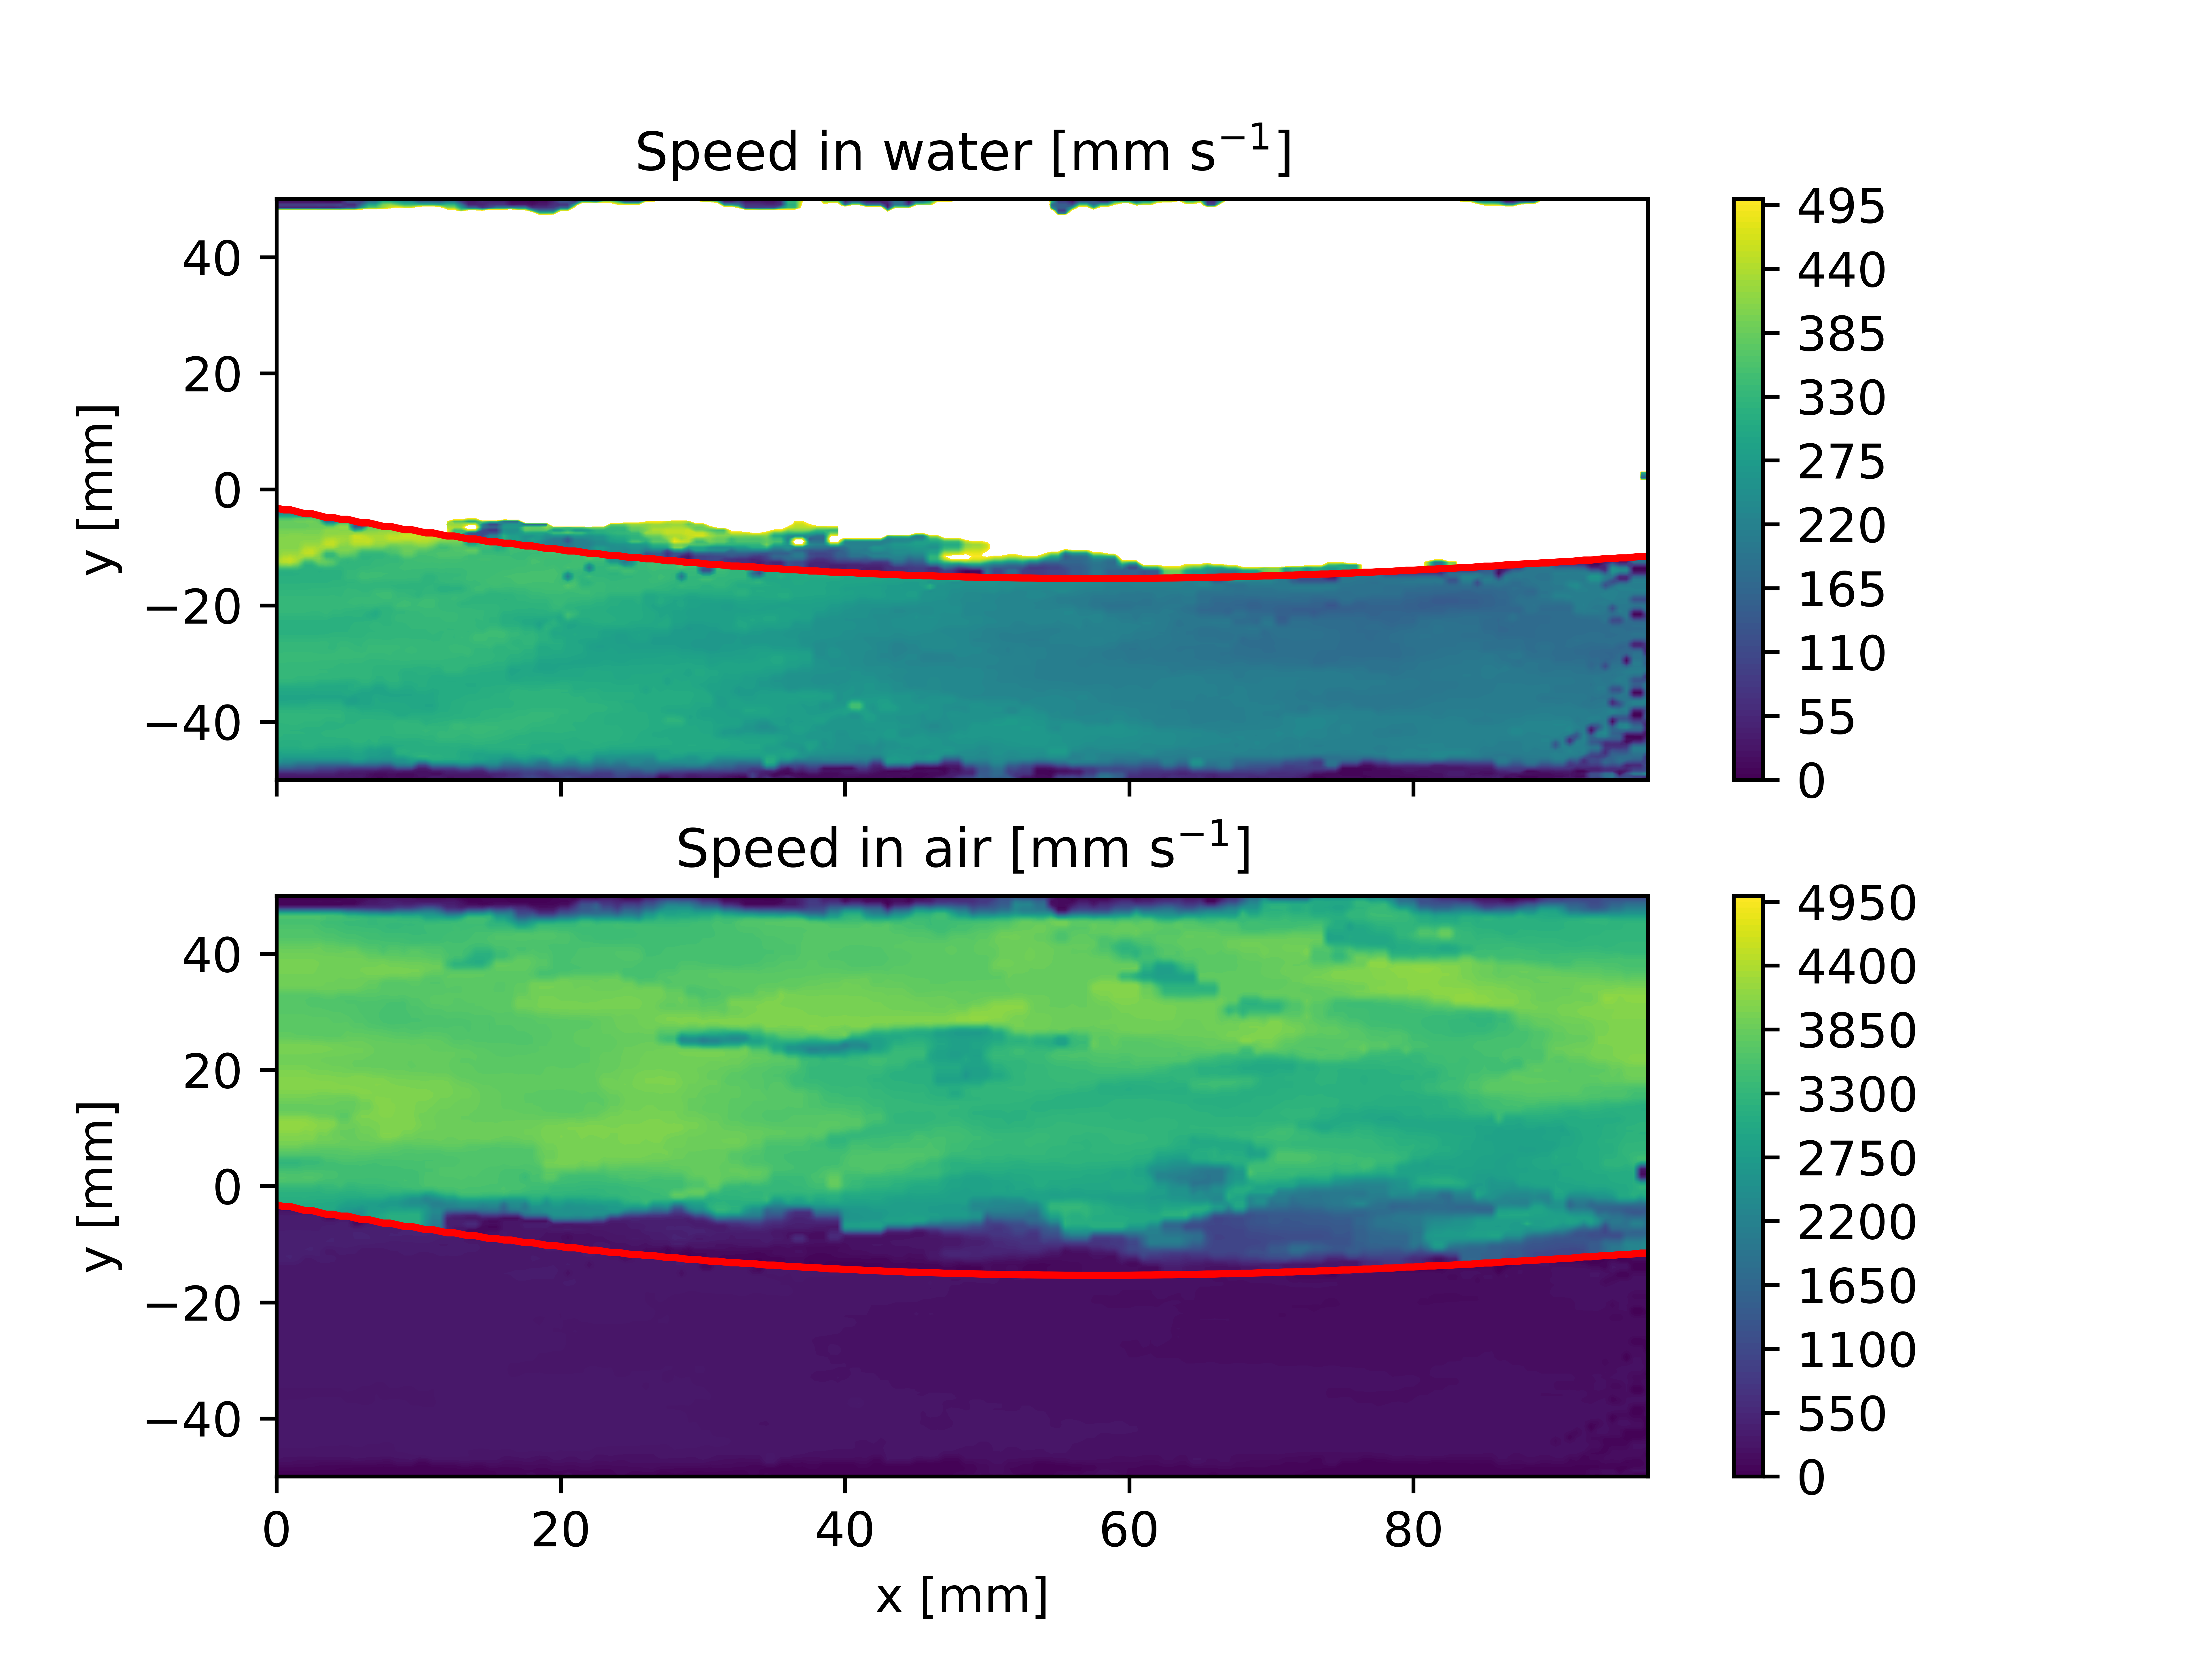
\includegraphics[scale=0.65]{../figures/task_b.png}
    \caption{Contour plot of $\sqrt{u^2 + v^2}$. Red line indicating border between gas and liquid.}
    \label{fig:contour_b}
\end{figure}

\begin{figure}[h!]
    \centering
    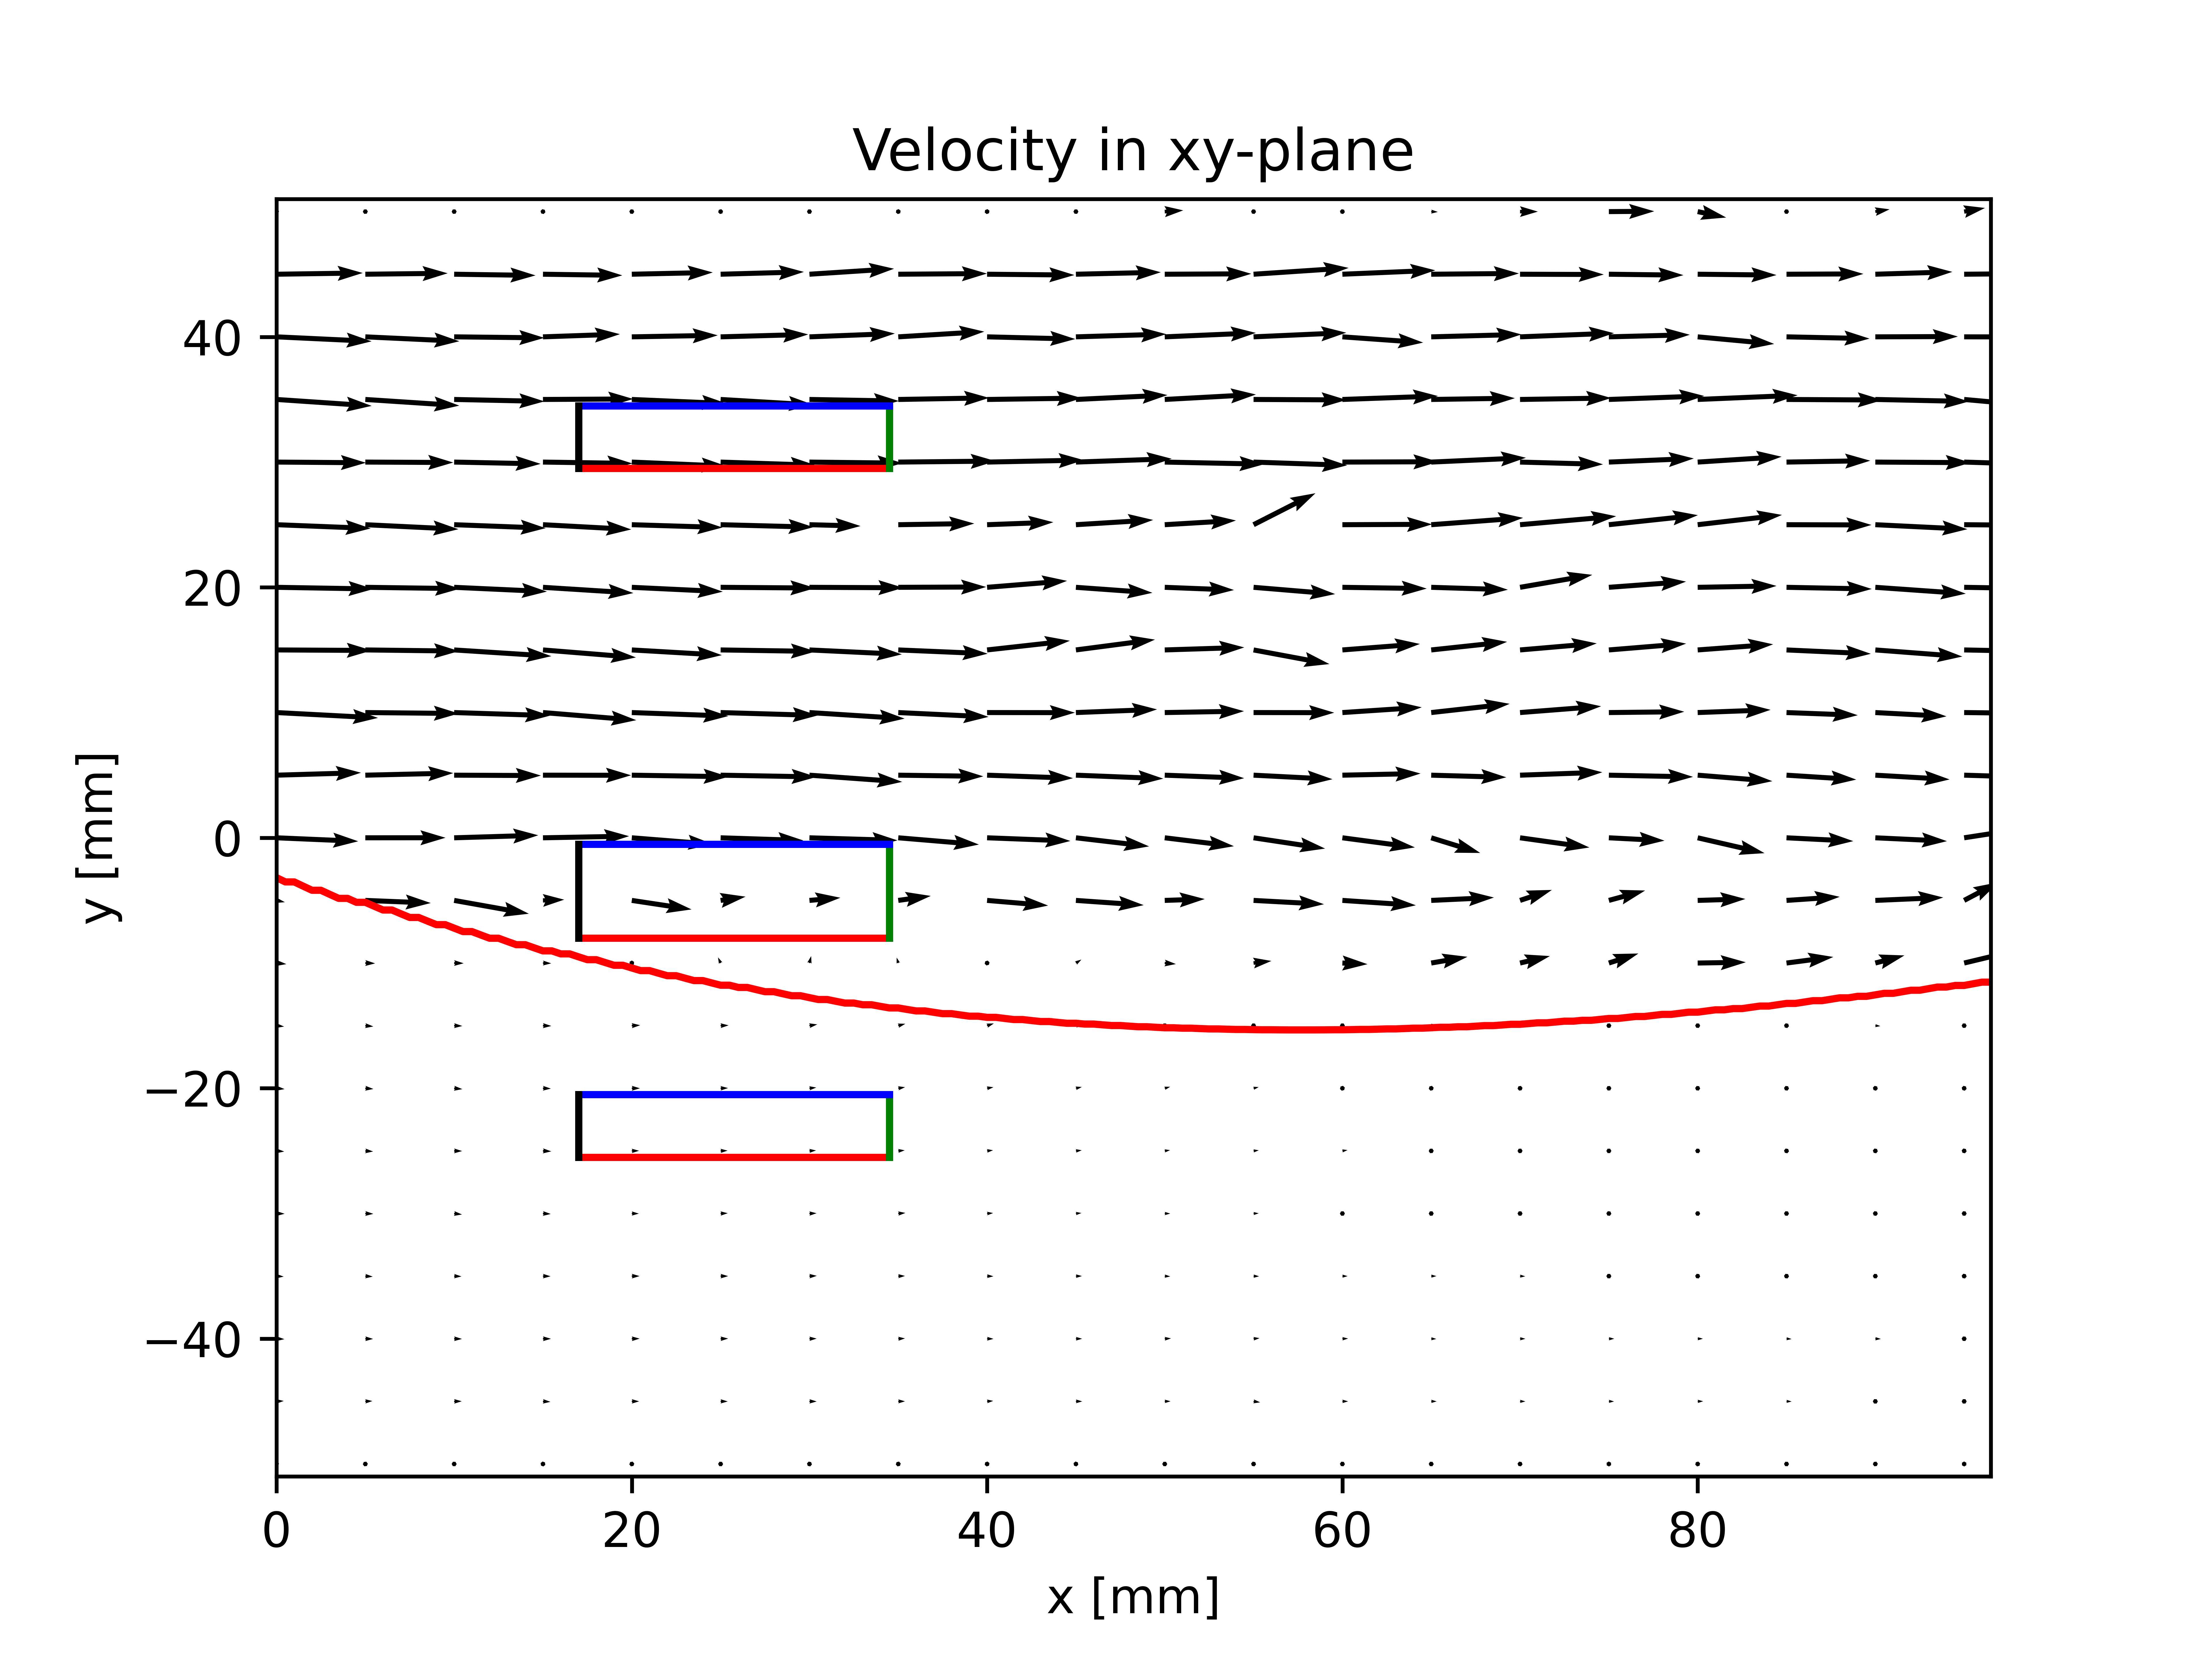
\includegraphics[scale=0.65]{../figures/task_c.png}
    \caption{Quiver plot of velocity $u\bm{i} + v\bm{j}$. Red line indicating border between gas and liquid.}
    \label{fig:quiver_c}
\end{figure}

\newpage
Let $\bm{v} = u\bm{i} + v\bm{j} + w\bm{k}$ and $\bm{v}^* = u\bm{i} + v\bm{j}$. The divergence is
\begin{align*}
    \mathbf{\nabla} \cdot \bm{v}^*
    = \frac{\partial u}{\partial x} + \frac{\partial v}{\partial y}
    \neq \mathbf{\nabla} \cdot \bm{v}
    = \frac{\partial u}{\partial x} + \frac{\partial v}{\partial y} + \frac{\partial w}{\partial z}
\end{align*}

\begin{figure}[h!]
    \centering
    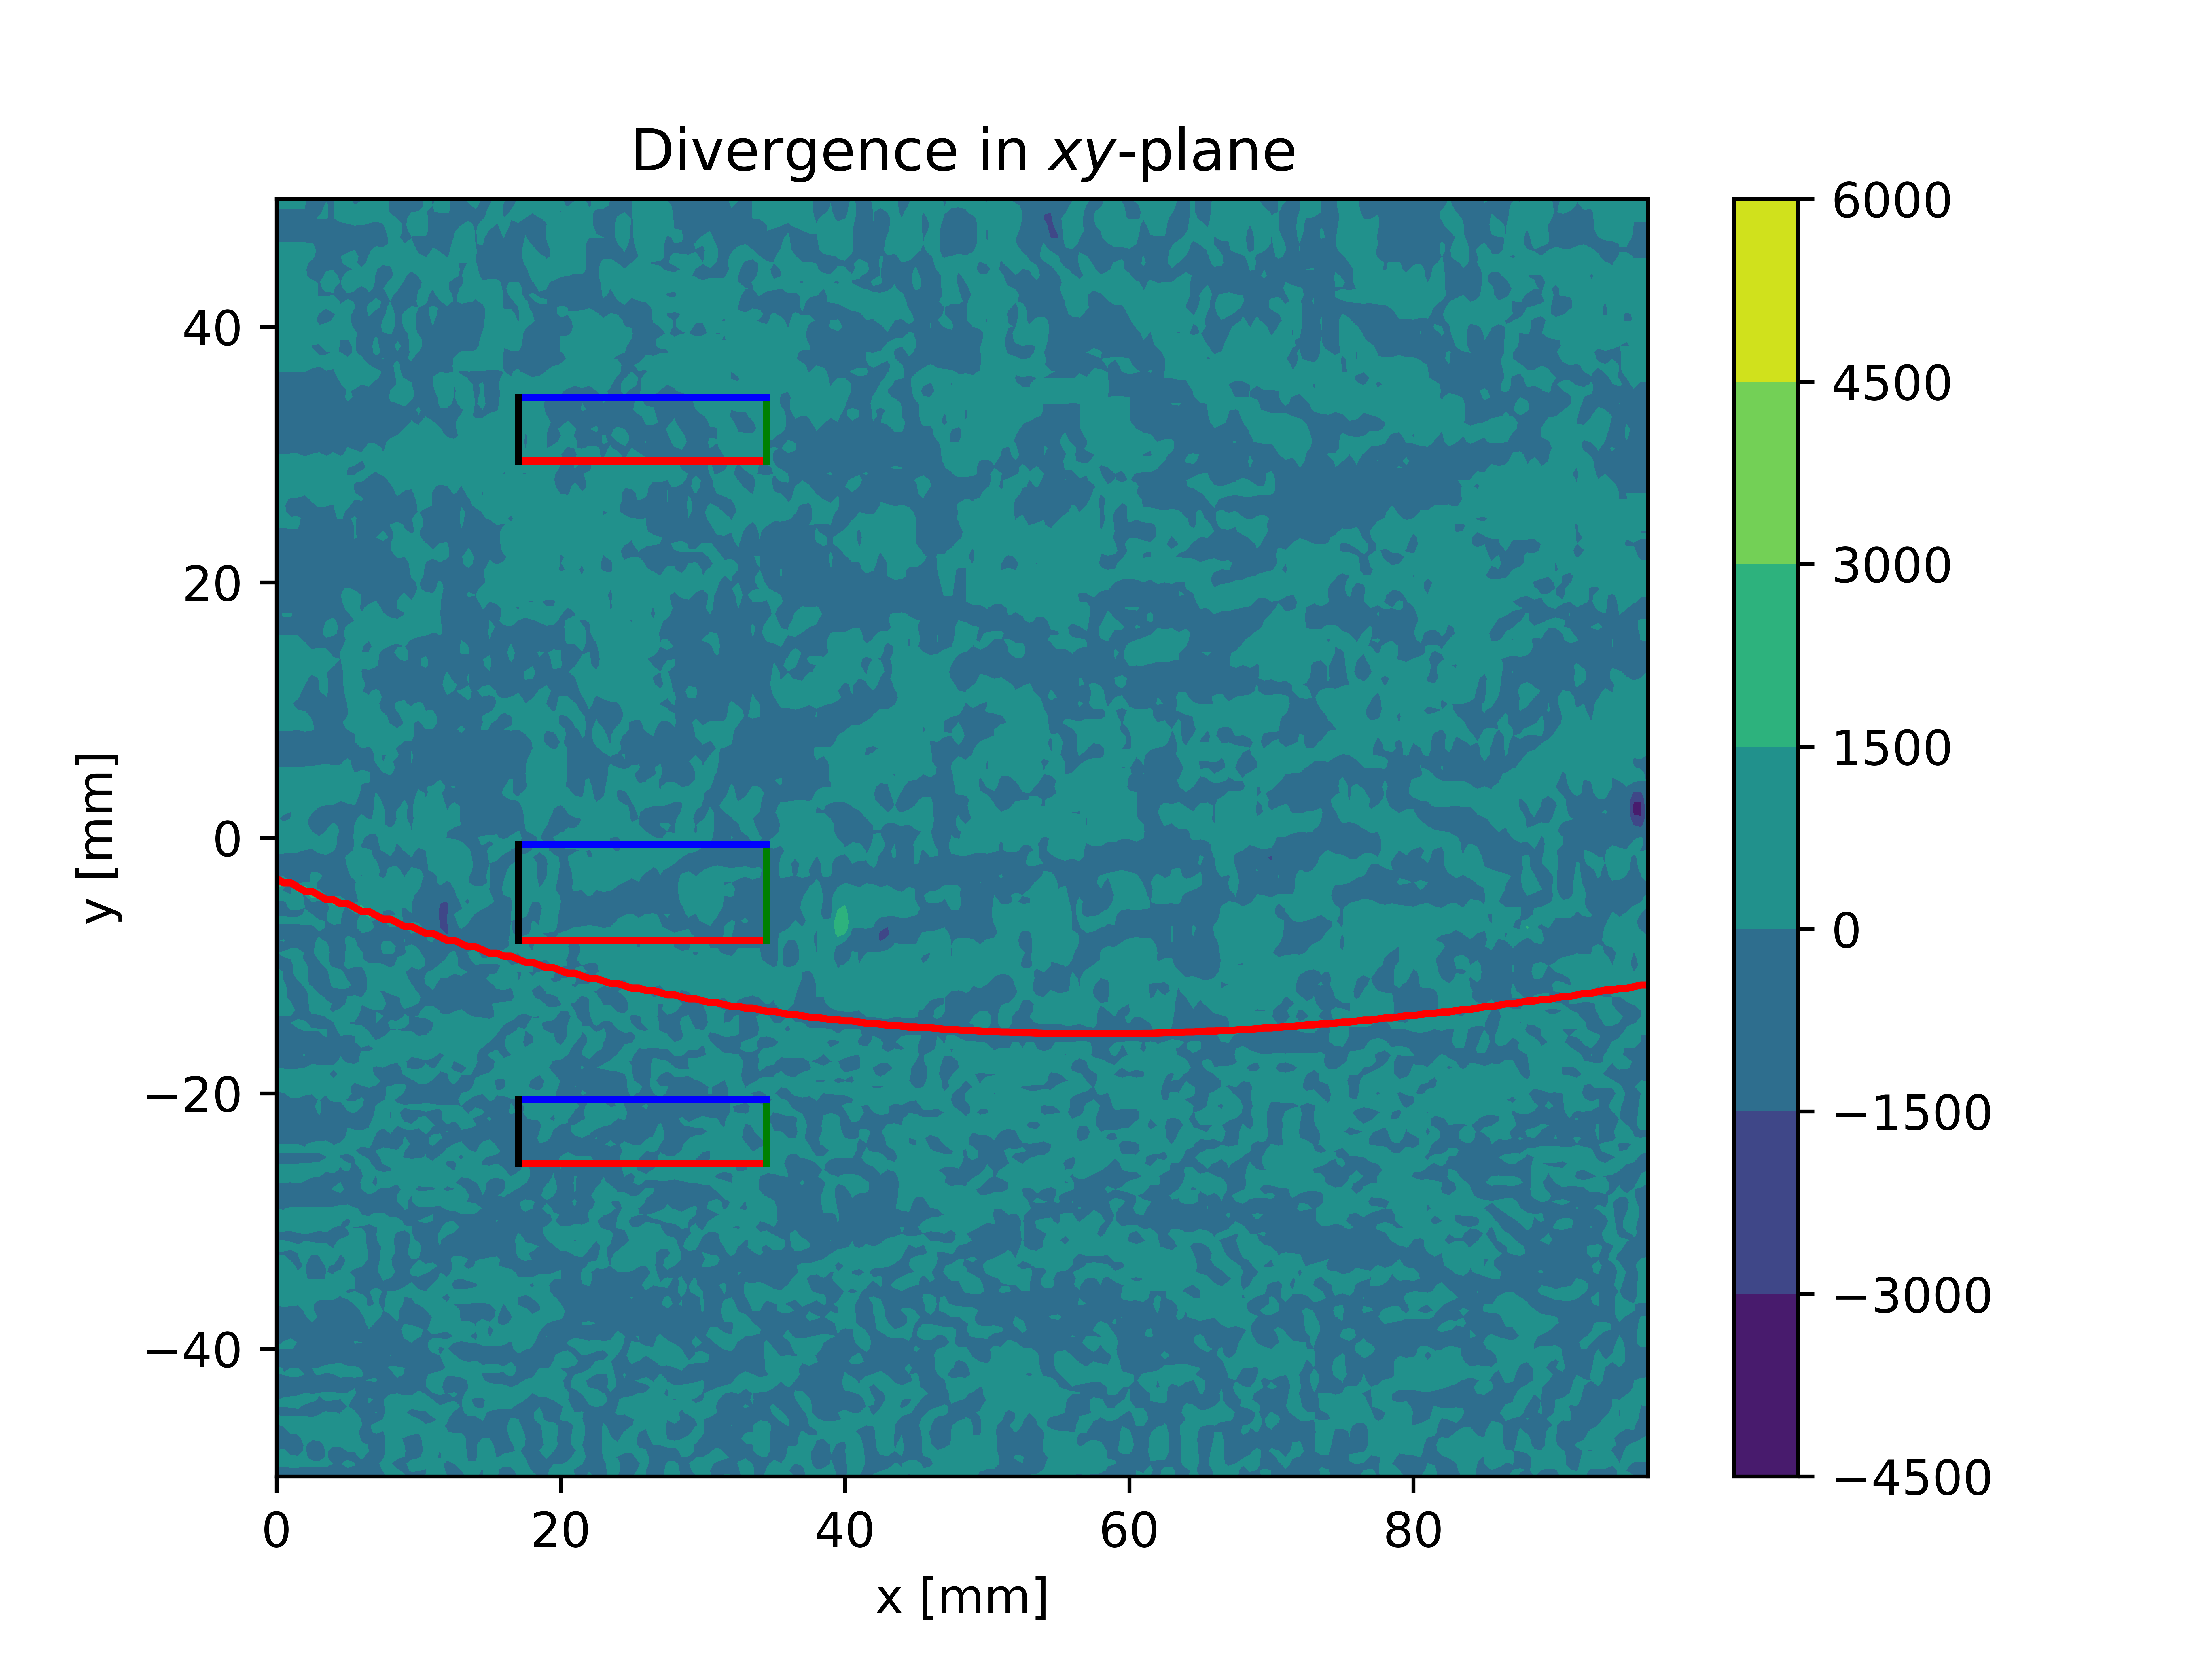
\includegraphics[scale=0.65]{../figures/task_d.png}
    \caption{Contour plot of $\nabla \cdot \bm{v}^*$. Red line indicating border between gas and liquid.}
    \label{fig:contour_d}
\end{figure}

Since both the gas and the liquid are modeled as incompressible fluids, the divergence should be zero. This means that 
\begin{align*}
    \mathbf{\nabla} \cdot \bm{v}
    &= \frac{\partial u}{\partial x} + \frac{\partial v}{\partial y} + \frac{\partial w}{\partial z}
    = 0 \\
    \implies \frac{\partial w}{\partial z}
    &= - \left(
            \frac{\partial u}{\partial x} + \frac{\partial v}{\partial y}
    \right) \\
    \implies w 
    &= - \int \left(
        \frac{\partial u}{\partial x} + \frac{\partial v}{\partial y}
    \right) dz.
\end{align*}

\begin{figure}[h!]
    \centering
    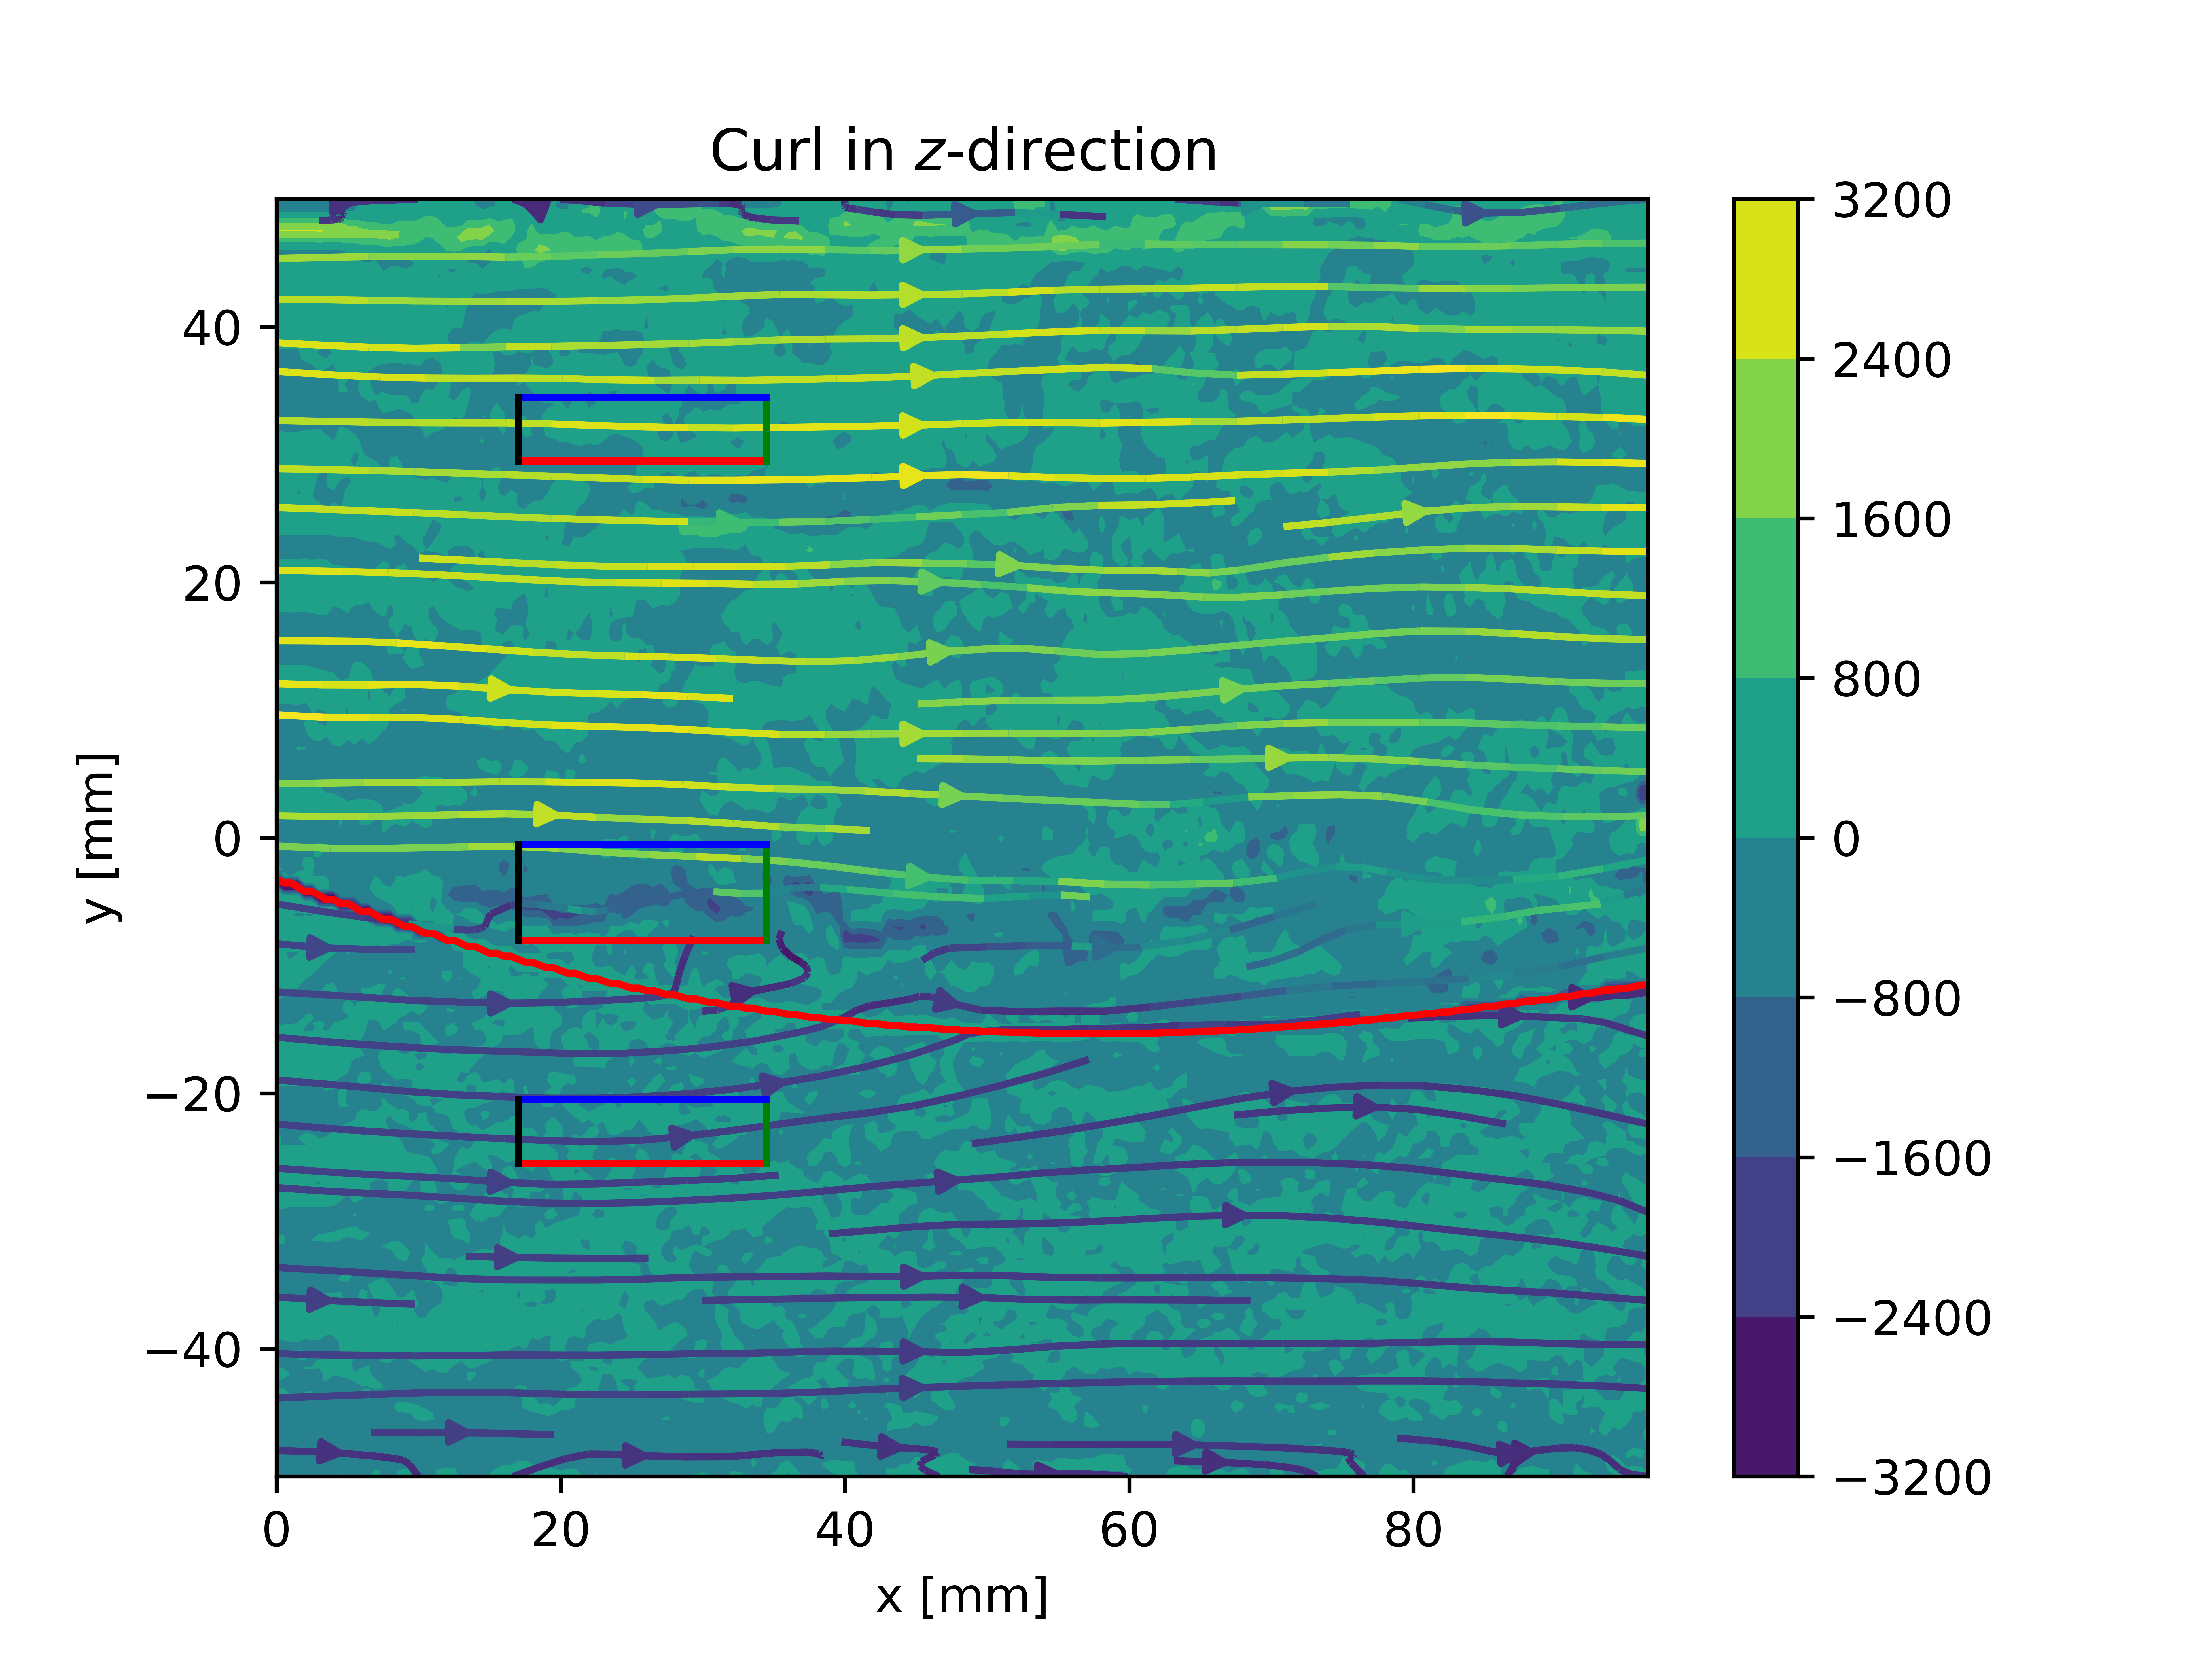
\includegraphics[scale=0.65]{../figures/task_e.png}
    \caption{Contour plot of $(\nabla \times \bm{v}^*) \cdot \bm{k}$. Red line indicating border between gas and liquid.}
    \label{fig:contour_e}
\end{figure}

BLABLA forklaring oppg E
- Beskriv strømningen for både gassfasen og væskefasen. Legg spesielt merke til strømningen ved veggen.

\newpage
The code in $\verb|integration.py|$ yields the following result:
\lstinputlisting[numbers=none]{../integration_out.txt}

\newpage
BLABLA forklaring oppg F
- Diskuter forskjellen mellom de tre rektanglene.
- For å få en bedre forståelse av sirkulasjonen angir du verdien til kurveintegralene langs hver side av rektanglene. Passer disse resultatene med hva du hadde forventet når du ser på hastighetsfeltet i området?


BLABLA forklaring oppg G
- Diskuter hvilken implikasjon disse svarene har for den integrerte fluksen over rektanglene orientert i z-retning
- For å få en bedre forståelse av fluksen skal du angi verdien til kurveintegralene langs hver side av rektanglene. Passer disse resultatene med hva du hadde forventet når du ser på hastighetsfeltet i området


\newpage
File: $\verb|plots.py|$
\lstinputlisting{../plots.py}

File: $\verb|integration.py|$
\lstinputlisting{../integration.py}

\end{document}
